%!TEX TS-program = pdflatex
%!TEX TS-options = -shell-escape
\RequirePackage{fix-cm}


\newcommand{\obenlinks}{Übungen zur Vorlesung Informatik I}   % hier Name der Veranstaltung eintragen
\documentclass[%
  paper=a4,
  fontsize=10pt,
  ngerman
  ]{scrartcl}

% Basics für Codierung und Sprache
% ===========================================================
  \usepackage{shellesc}                 % Compiler-Option -shell-escape benutzen!
  \usepackage[final]{graphicx}          % Einbindung von Grafiken
  \usepackage{subcaption}
%  \usepackage[utf8]{inputenc}          % Dateien sind UTF8-codiert
  \usepackage{babel}                    % deutsche Silbentrennung, etc.
  \usepackage[german=quotes]{csquotes}  % deutsche Anführungszeichen mit \enquote{...}
% ===========================================================

% Fonts und Typographie
% ===========================================================
  \usepackage[babel=true,final,tracking=smallcaps]{microtype}
  \DisableLigatures{encoding = T1, family = tt* }   % keine Ligaturen für Monospace-Fonts
% ===========================================================

% Farben
% ===========================================================
  \usepackage[usenames,x11names,final]{xcolor}
% ===========================================================

% Mathe-Pakete und -Einstellungen
% ===========================================================
  \usepackage{mathtools}               % Tools zum Setzen von Formeln
  \usepackage{amssymb}                 % übliche Mathe-Symbole
  \usepackage[bigdelims]{newtxmath}    % moderne Mathe-Font
  \allowdisplaybreaks                  % seitenübergreifende Rechnungen
  \usepackage{bm}                      % math bold font
  \usepackage{wasysym}                 % noch mehr Symbole
% ===========================================================

% TikZ
% ===========================================================
  \usepackage{tikz}
  \usetikzlibrary{arrows,arrows.meta}    % mehr Pfeile!
  \usetikzlibrary{calc}                  % TikZ kann rechnen
  \usetikzlibrary{positioning}
  \tikzset{>=Latex}                      % Standard-Pfeilspitze
% ===========================================================

% Seitenlayout, Kopf-/Fußzeile
% ===========================================================
  \usepackage{scrlayer-scrpage}
  \pagestyle{scrheadings}
  \usepackage[top=5cm, bottom=3cm, left=2.5cm, right=2cm]{geometry}
  \clearscrheadfoot 
  \setheadsepline{0.4pt}                            % Linie in Kopfzeile
  \setfootsepline{0.4pt}                            % Linie in Fußzeile
  \setkomafont{section}{\fontsize{14bp}{18.8bp}\normalfont}  % Schriftart der Section
  \setkomafont{subsection}{\fontsize{12bp}{16bp}\normalfont}                  
  \setkomafont{pagehead}{\textnormal}                 % Schriftart Kopfzeile
  \setkomafont{pagefoot}{\normalfont\footnotesize}  % Schriftart Fußzeile 
  \cfoot{\thepage}                                  % Seitenzahl unten Mitte
  \lohead{\obenlinks}                               % Titel oben links
  \raggedbottom                                     % Flattersatz
  \usepackage{setspace}                             % erweiterte Abstandsoptionen
  \onehalfspacing                                   % Zeilenabstand 1.5-fach
  \setlength{\parindent}{0pt}                       % Einrückung neuer Absätze
  \setlength{\parskip}{0.5\baselineskip}            % Abstand neuer Absätze
% ===========================================================

% Hyperref für Referenzen und Hyperlinks
% ===========================================================
  \usepackage[%
    hidelinks,
    pdfpagelabels,
    bookmarksopen=true,
    bookmarksnumbered=true,
    linkcolor=black,
    urlcolor=SkyBlue2,
    plainpages=false,
    pagebackref,
    citecolor=black,
    hypertexnames=true,
    pdfborderstyle={/S/U},
    linkbordercolor=SkyBlue2,
    colorlinks=false,
    backref=false]{hyperref}
  \hypersetup{final}
% ===========================================================

% Listen und Tabellen
% ===========================================================
  \usepackage{multicol}
  \usepackage[shortlabels]{enumitem}
  \setlist{itemsep=0pt}
  \setlist[enumerate]{font=\sffamily\bfseries}
  \setlist[itemize]{label=$\triangleright$}
  \usepackage{tabularx}
% ===========================================================

% minted
% ===========================================================
\usepackage{minted}
\setminted{%
  style=default,
  fontsize=\small,
  breaklines,
  breakanywhere=false,
  breakbytoken=false,
  breakbytokenanywhere=false,
  breakafter={.,},
  autogobble,
  numbersep=3mm,
  tabsize=4,
  linenos,
  frame=lines
}
\setmintedinline{%
  fontsize=\normalsize,
  numbers=none,
  numbersep=12pt,
  tabsize=4,
}

%%%%%%%%%%%%%%%%%%%%%%%%%%%%%%%%%%%%%%%%%%%%%%%%%%%%%%%%%%%
%%% Ab hier folgen nur noch vordefinierte Mathe-Befehle %%%
%%%%%%%%%%%%%%%%%%%%%%%%%%%%%%%%%%%%%%%%%%%%%%%%%%%%%%%%%%%

\newcommand{\BB}{\mathbb{B}}
\newcommand{\CC}{\mathbb{C}}
\newcommand{\NN}{\mathbb{N}}
\newcommand{\QQ}{\mathbb{Q}}
\newcommand{\RR}{\mathbb{R}}
\newcommand{\ZZ}{\mathbb{Z}}
\newcommand{\oh}{\mathcal{O}}            
\newcommand{\ol}[1]{\overline{#1}}
\newcommand{\wt}[1]{\widetilde{#1}}
\newcommand{\wh}[1]{\widehat{#1}}

\DeclareMathOperator{\id}{id}                        % Identität
\DeclareMathOperator{\pot}{\mathcal{P}}              % Potenzmenge

% Klammerungen und ähnliches
\DeclarePairedDelimiter{\absolut}{\lvert}{\rvert}    % Betrag
\DeclarePairedDelimiter{\ceiling}{\lceil}{\rceil}    % aufrunden
\DeclarePairedDelimiter{\Floor}{\lfloor}{\rfloor}    % aufrunden
\DeclarePairedDelimiter{\Norm}{\lVert}{\rVert}       % Norm
\DeclarePairedDelimiter{\sprod}{\langle}{\rangle}    % spitze Klammern
\DeclarePairedDelimiter{\enbrace}{(}{)}              % runde Klammern
\DeclarePairedDelimiter{\benbrace}{\lbrack}{\rbrack} % eckige Klammern
\DeclarePairedDelimiter{\penbrace}{\{}{\}}           % geschweifte Klammern
\newcommand{\Underbrace}[2]{{\underbrace{#1}_{#2}}}  % bessere Unterklammerungen
% Kurzschreibweisen für Faule und Code-Vervollständigung
\newcommand{\abs}[1]{\absolut*{#1}}
\newcommand{\ceil}[1]{\ceiling*{#1}}
\newcommand{\flo}[1]{\Floor*{#1}}
\newcommand{\no}[1]{\Norm*{#1}}
\newcommand{\sk}[1]{\sprod*{#1}}
\newcommand{\enb}[1]{\enbrace*{#1}}
\newcommand{\penb}[1]{\penbrace*{#1}}
\newcommand{\benb}[1]{\benbrace*{#1}}
\newcommand{\stack}[2]{\makebox[1cm][c]{$\stackrel{#1}{#2}$}}  % Präambel (ohne die geht nichts!)
\ihead{
  \section*{Informatik I - Gruppe 1 - Übungblatt 3}
  
  Ausgabe: 31.10.2022

  Abgabe: 07.11.2022

  Tutor: Tim Völker

  ~
}

\ohead{

  ~

  ~

  ~

  Ali Kurt 528961

  Thomas Kujawa 463620

  Felix Hoff 374689

  ~
}


\begin{document}
\graphicspath{ {./images/} }
\textbf{Aufgabe T3.1:} Interpretation von Numeralen \textit{(1.5+1.5+2=5 Punkte)}

In der Vorlesung haben Sie eine induktive Definition von arithmetischen Ausdrücken über den natürlichen Zahlen kennengelernt. Modifizieren Sie die Interpretationsvorschrift, so dass folgende Zuordnungen für Numerale stattfinden:

\begin{itemize}
  \item[(a)] $234 \in N \rightarrow a(234)=9 \in \mathbb{N}_{0}$ (Quersumme)

$$
\begin{aligned}
& z \in Z \Rightarrow a(z)=z \\
& n \in N \wedge z \in Z \Rightarrow a(n z)=a(n)+a(z)
\end{aligned}
$$
Für 234
$$
\begin{aligned}
& a(234)=a(23)+a(4) \\
& a(23)=a(2)+a(3) \\
&(a(2)+a(3))+a(4)=2+3+4=9
\end{aligned}
$$

  \item[(b)] $123 \in N \rightarrow a(123)=3 \in \mathbb{N}_{0}$ (Letzte Ziffer)

  $$
  \begin{aligned}
  &z \in Z \Rightarrow a(z)=z\\
  &n \in N_{\wedge} z \in z \Rightarrow a(n z)=a(z)
  \end{aligned}
  $$
  Für 123
  $$
  \begin{aligned}
  &a(123)=a(3)=3
\end{aligned}
$$

  \item[(c)] $12345 \in N \rightarrow a(12345)=2 \in \mathbb{N}_{0}$ (Anzahl gerader Ziffern)
  
  $$
\begin{aligned}
& z \in\{0,2,4,6,8\} \Rightarrow a(z)=1 \\
& z \in\{1,3,5,7,9\} \Rightarrow a(z)=0 \\
& z \in Z \land n \in N \Rightarrow a(n z)=a(n)+a(z) \\
\end{aligned}
$$

Für 12345

$$
\begin{aligned}
& a(12345)=a(1234)+a(5) \quad \rightarrow a(5)=0 \\
& a(1234)=a(123)+a(4) \quad\quad \rightarrow a(4)=1 \\
& a(123)=a(12)+a(3) \quad\quad \rightarrow a(3)=0 \\
& \cdots \rightarrow a(1)+a(2)+a(3)+a(4)+a(5)=2
\end{aligned}
$$

\end{itemize}

\newpage

\textbf{Aufgabe T3.2:} Hierarchische Struktur \textit{(3+1+1=5 Punkte)} 

Im Folgenden sollen verschiedene Darstellungen arithmetischer Ausdrücke mit den Operatoren $*,+$, : und - geübt werden.

\begin{itemize}
  \item [(a)] Überführen Sie den Term $\frac{\frac{1}{4} x-y(z-1)}{y-z^{2}}$ in einen arithmetischen Ausdruck und skizzieren Sie die zugehörige Baumdarstellung.
  
  $$
  \textcolor{red}{(}\textcolor{blue}{(}\textcolor{green}{(}(1 / 4) \textcolor{green}{*} \mathrm{x}\textcolor{green}{)}-\textcolor{green}{(}\mathrm{y} \textcolor{green}{*}(\mathrm{z}-1)\textcolor{green}{)}\textcolor{blue}{)} \textcolor{red}{/}\textcolor{blue}{(}\mathrm{y}-\textcolor{green}{(}\mathrm{z} \textcolor{green}{*} \mathrm{z}\textcolor{green}{)}\textcolor{blue}{)}\textcolor{red}{)}
  $$
  
  \begin{center}
  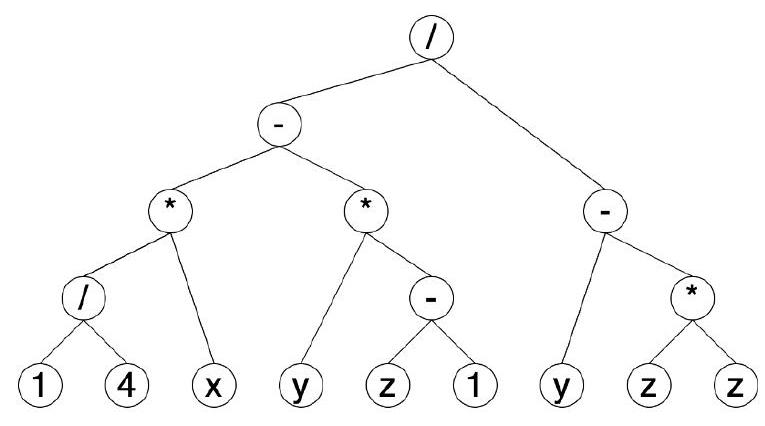
\includegraphics[width=10cm]{2023_01_23_87b3ed9af9e71cf7f31ag-1}
  \end{center}
  
  \item [(b)] Leiten Sie von der Baumdarstellung aus (a) eine Präfix-Notation des Terms ab. Heben Sie die Teilbäume durch Klammerungen in ihrem Ausdruck hervor.
  
  $$
  \textcolor{red}{(/}\textcolor{blue}{(-}\textcolor{green}{(*}(/ 14) \mathrm{x}\textcolor{green}{)(*} \mathrm{y}(-\mathrm{z} 1)\textcolor{green}{)}\textcolor{blue}{)(}-\mathrm{y}\textcolor{green}{(*} \mathrm{z} \mathrm{z}\textcolor{green}{)}\textcolor{blue}{)}\textcolor{red}{)}
  $$

  \item [(c)] Gegeben sei der folgende Term in Infix-Notation:
  
  $((a *(b / c)) *(a+b)-(c+2 * a)) /((b+c) *(b+c))$
  
  Schreiben Sie den Term in Präfix-Notation um.

  $$
  \textcolor{red}{(/}\textcolor{blue}{(-}\textcolor{green}{(*}\textcolor{red}{(*} \mathrm{a}(/ \mathrm{b} \mathrm{c})\textcolor{red}{)(+}\mathrm{ab}\textcolor{red}{)}\textcolor{green}{)(+}\mathrm{c}\textcolor{red}{(*} 2 \mathrm{a}\textcolor{red}{)}\textcolor{green}{)}\textcolor{blue}{)(*}\textcolor{green}{(+}\mathrm{bc}\textcolor{green}{)(+}\mathrm{bc}\textcolor{green}{)}\textcolor{blue}{)}\textcolor{red}{)}
  $$
\end{itemize}

\newpage

\textbf{Aufgabe P3.3:} Programmentwurf: Umrechnen von Distanzen \textit{(5 Punkte)} 

Erstellen Sie Programme, die eine Distanz in Kilometern umrechnet in die äquivalente Distanz in Meilen und umgekehrt, und implementieren Sie sie in Haskell. Folgen Sie dabei dem Programmentwurf der Vorlesung und erstellen Sie (1) Funktionsköpfe, (2) Beispiele und (3) Funktionsrümpfe sowie (4) eine Überprüfung anhand der generierten Beispiele.

\textit{Hinweise:}
\begin{itemize}
  \item [•] Geben Sie die Beispiele als Kommentar in Ihrem Quellcode mit ab.

  \item [•] Schlagen Sie gegebenenfalls benötigte Formeln nach.
\end{itemize}

\begin{itemize}
  \item [] \inputminted{Haskell}{P3_3.hs}
\end{itemize}

\newpage

\textbf{Aufgabe P3.4:} Programmentwurf: Unixzeit \textit{(3+3.5+3.5=10 Punkte)}

Die Unixzeit ist eine Zeitrechnung, die die Sekunden zählt, die seit Donnerstag, dem 1. Januar 1970, 00:00 Uhr UTC vergangen sind. Die Unixzeit wird häufig für Zeitstempel verwendet und kann in unsere normale Datumsdarstellung umgewandelt werden.

\begin{itemize}
  \item [(a)] Erstellen Sie ein Programm, das aus der Unixzeit berechnet, wie viele Sekunden am aktuellen Tag seit Mitternacht (UTC) vergangen sind.

  \item [(b)] Erstellen Sie ein Programm, das zwei Unixzeiten entgegen nimmt und bestimmt, wie viele ganze Tage zwischen den beiden Zeitpunkten vergangen sind.  \item [(c)] Erstellen Sie ein Programm, das aus der Unixzeit berechnet, wie viele volle Stunden in Deutschland (Winterzeit) am aktuellen Tag vergangen sind, z.B. sind um 15:25 Uhr bereits 15 volle Stunden vergangen.
\end{itemize}


Folgen Sie dabei dem Programmentwurf der Vorlesung und erstellen Sie (1) Funktionskopf, (2) Beispiele und (3) Funktionsrumpf sowie (4) eine Überprüfung anhand der generierten Beispiele. Implementieren Sie die Programme in Haskell.

\textit{Hinweise:}

\begin{itemize}
  \item [•] Für die Modulo-Berechnung können Sie in Haskell die Funktion \mintinline{Haskell}{mod : : Integer -> Integer -> Integer} verwenden.

  \item [•] Für die Ganzzahl-Division können Sie in Haskell die Funktion \mintinline{Haskell}{div :: Integer -> Integer -> Integer} verwenden.

  \item [•] Geben Sie die Beispiele als Kommentar in Ihrem Quellcode mit ab.

  \item [•] Schlagen Sie gegebenenfalls benötigte Informationen zur Umrechnung nach.
\end{itemize}

\newpage

\begin{itemize}
  \item [] \inputminted{Haskell}{P3_4.hs}
\end{itemize}
\end{document}